\section{Auswertung}
\label{sec:Auswertung}

\subsection{Bestimmung der Wellenlänge des Laserlichtes}

Zur Bestimmung der Wellenlänge des Laserlichtes wird die Formel \eqref{eqn:2} aus der Theorie verwendet.
Daher wird die Wellenlänge nach
\begin{equation}
  \lambda = 2\frac{\Delta l}{N}
\end{equation}
berechnet.
Dabei steht $\Delta l$ für die Verschiebung des Spiegels ausgelöst durch den Motor und $N$ für die gezählten Maxima des Interferenzmusters, die den Detektor während der Verschiebung passieren.
Die zusätzliche Wegstrecke wird über eine Verschiebung des Spiegels um die Länge $\increment{x}$ realisiert, die mit einer Übersetzung von $5.046:1$ in $\increment{l}$ umgesetzt wird.
Die Ergebnisse der Messung sind in Tabelle \ref{tab:1} einzusehen.

\begin{table}
    \centering
    \caption{Messdaten zur Bestimmung der Ablenkung im B-Feld.}
    \label{table:A2}
    \sisetup{parse-numbers=false}
    \begin{tabular}{
	S[table-format=1.2]
	S[table-format=1.2]
	S[table-format=1.2]
	S[table-format=1.2]
	S[table-format=1.2]
	S[table-format=1.2]
	}
	\toprule
	{$D \:/\: \text{in}$}		& {$I_1 \:/\: \si{\ampere}$}		& 
	{$I_2 \:/\: \si{\ampere}$}		& {$I_3 \:/\: \si{\ampere}$}		& 
	{$I_4 \:/\: \si{\ampere}$}		& {$I_5 \:/\: \si{\ampere}$}		\\ 
	\midrule
    0.00 & 0.00 & 0.00 & 0.00 & 0.00 & 0.00 \\
0.25 & 0.28 & 0.30 & 0.32 & 0.35 & 0.40 \\
0.50 & 0.58 & 0.64 & 0.69 & 0.74 & 0.81 \\
0.75 & 0.89 & 1.00 & 1.07 & 1.14 & 1.25 \\
1.00 & 1.19 & 1.34 & 1.44 & 1.56 & 1.66 \\
1.25 & 1.52 & 1.68 & 1.81 & 1.94 & 2.09 \\
1.50 & 1.84 & 2.20 & 2.20 & 2.34 & 1.51 \\
1.75 & 2.18 & 2.39 & 2.58 & 2.75 & 2.94 \\
2.00 & 2.49 & 2.73 & 2.95 & /    & /    \\

    \bottomrule
    \end{tabular}
    \end{table}


%Da der siebte und achte Wert offensichtlich nicht reinpassen... raus
Die Wellenlänge wird nach den Formeln \eqref{eq:std} und \eqref{eq:std_mean} auf den Wert
\begin{align*}
  \lambda_{\text{Laser}} = \input{build/lambda_laser.tex}
\end{align*}
gemittelt.

\subsection{Bestimmung der Brechungsindizes von Gasen}

Im Folgenden wird zur Berechnung des Brechungsindex die Formel
\begin{equation}
  n(p_0,T_0) = 1 +\Delta n(\Delta p) \frac{T}{T_0}\frac{p_0}{\Delta p}
\end{equation}
verwendet, bei der $p_0$ den Normaldruck und $T_0$ die Normaltemperatur beschreibt.
Wird diese Formel durch den Ausdruck (\ref{eqn:3}) ergänzt ergibt sich
\begin{equation}
  n(p_0,T_0) = 1 +\frac{N \lambda}{2b} \frac{T}{T_0}\frac{p_0}{\Delta p},
\end{equation}
wobei $\lambda$ die zuvor bestimmte Wellenlänge des Lasers und $b$ die Länge des Gasbehälters ist, welchen das Laserlicht passiert.
Die Konstanten dieses Experiments betragen
\begin{align*}
  p_0 &= \SI{1013,2}{\milli\bar},\\
  T_0 &= \SI{273,15}{\kelvin} \: \text{und}\\
  b   &= \SI{50}{\milli\metre}.\\
\end{align*}
Die Messwerte und entsprechenden Ergebnisse der Messung des Brechungsindex von Luft sind in Tabelle \ref{tab:2} aufgeführt.

\begin{table}
    \centering
    \caption{Messdaten zur Bestimmung der Ablenkung im E-Feld.}
    \label{table:b}
    \sisetup{parse-numbers=false}
    \begin{tabular}{
	S[table-format=1.2]
	S[table-format=4.2]
	S[table-format=4.2]
	S[table-format=4.2]
	S[table-format=4.2]
	S[table-format=4.2]
	}
	\toprule
	{$D \:/\: \text{in}$}		& {$U_1 \:/\: \si{\volt}$}		&
	{$U_2 \:/\: \si{\volt}$}		& {$U_3 \:/\: \si{\volt}$}		&
	{$U_4 \:/\: \si{\volt}$}		& {$U_5 \:/\: \si{\volt}$}		\\
	\midrule
    0.00 & -8.55 & -11.09 & -13.35 & -14.23 & -17.43 \\
0.25 & -4.58 & -6.36  & -7.82  & -7.67  & -10.13 \\
0.50 & -1.10 & -1.87  & -1.96  & -1.06  & -2.40  \\
0.75 & 2.61  & 2.91   & 3.79   & 5.38   & 5.17   \\
1.00 & 6.18  & 7.59   & 8.92   & 11.67  & 12.58  \\
1.25 & 9.59  & 12.00  & 14.64  & 17.93  & 19.83  \\
1.50 & 13.26 & 16.60  & 20.09  & 24.32  & 27.00  \\
1.75 & 16.80 & 20.98  & 25.31  & 30.78  & 34.23  \\
2.00 & 20.40 & 25.35  & 30.81  & /      & /      \\

    \bottomrule
    \end{tabular}
    \end{table}


Gemittelt ergibt sich daher für den Brechungsindex von Luft der Wert
\begin{align*}
  n_{\text{Luft}} = \input{build/n_luft.tex}, \label{luft}
\end{align*}
wobei für die Fehlerrechnung die Gaußsche Fehlerfortpflanzung (\ref{gauss}) verwendet wurde.

Die Messergebnisse für $\ce{C4H8}$ sind in Tabelle \ref{tab:3} dargestellt.

\begin{table}
    \centering
    \caption{Fitparameter: Steigung $m$ und y-Achsenabschnitt $b$.}
    \label{tab:c}
    \sisetup{parse-numbers=false}
    \begin{tabular}{
	S[table-format=3.0]
	S[table-format=2.2]
	S[table-format=1.2]
	S[table-format=2.2]
	S[table-format=1.2]
	}
	\toprule
	{$U_b \:/\: \si{\volt}$}		& {$m \:/\: 10^{-4}\si{\metre\per\volt}$}		& 
	{$\increment{m} \:/\: 10^{-4}\si{\metre\per\volt}$}		& {$b \:/\: 10^{-3}\si{\volt}$}		& 
	{$\increment{b} \:/\: 10^{-3}\si{\volt}$}		\\ 
	\midrule
    17.67 & 0.08 & 14.68 & 0.09 \\
13.91 & 0.07 & 15.18 & 0.09 \\
11.51 & 0.06 & 15.11 & 0.10 \\
9.91  & 0.03 & 13.91 & 0.06 \\
8.58  & 0.04 & 14.84 & 0.08 \\

    \bottomrule
    \end{tabular}
    \end{table}


Daraus lässt sich ein Mittelwert von
\begin{align*}
  n_{\ce{C4H8}} = \input{build/n_gas.tex}\\
\end{align*}
berechnen.



















% % Examples
% \begin{equation}
%   U(t) = a \sin(b t + c) + d
% \end{equation}
%
% \begin{align}
%   a &= \input{build/a.tex} \\
%   b &= \input{build/b.tex} \\
%   c &= \input{build/c.tex} \\
%   d &= \input{build/d.tex} .
% \end{align}
% Die Messdaten und das Ergebnis des Fits sind in Abbildung~\ref{fig:plot} geplottet.
%
% %Tabelle mit Messdaten
% \begin{table}
%   \centering
%   \caption{Messdaten.}
%   \label{tab:data}
%   \sisetup{parse-numbers=false}
%   \begin{tabular}{
% % format 1.3 bedeutet eine Stelle vorm Komma, 3 danach
%     S[table-format=1.3]
%     S[table-format=-1.2]
%     @{${}\pm{}$}
%     S[table-format=1.2]
%     @{\hspace*{3em}\hspace*{\tabcolsep}}
%     S[table-format=1.3]
%     S[table-format=-1.2]
%     @{${}\pm{}$}
%     S[table-format=1.2]
%   }
%     \toprule
%     {$t \:/\: \si{\milli\second}$} & \multicolumn{2}{c}{$U \:/\: \si{\kilo\volt}$\hspace*{3em}} &
%     {$t \:/\: \si{\milli\second}$} & \multicolumn{2}{c}{$U \:/\: \si{\kilo\volt}$} \\
%     \midrule
%     \input{build/table.tex}
%     \bottomrule
%   \end{tabular}
% \end{table}
%
% % Standard Plot
% \begin{figure}
%   \centering
%   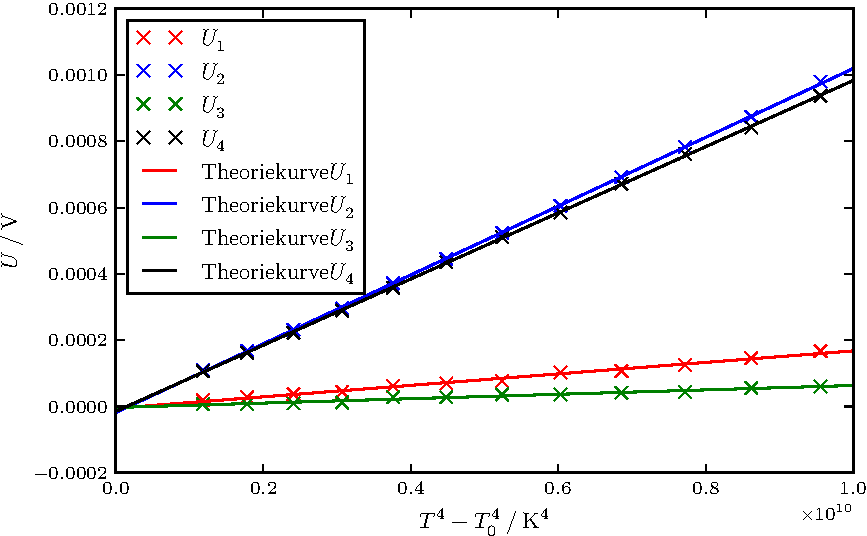
\includegraphics{build/plot.pdf}
%   \caption{Messdaten und Fitergebnis.}
%   \label{fig:plot}
% \end{figure}
%
% 2x2 Plot
% \begin{figure*}
%     \centering
%     \begin{subfigure}[b]{0.475\textwidth}
%         \centering
%         \includegraphics[width=\textwidth]{Abbildungen/Schaltung1.pdf}
%         \caption[]%
%         {{\small Schaltung 1.}}
%         \label{fig:Schaltung1}
%     \end{subfigure}
%     \hfill
%     \begin{subfigure}[b]{0.475\textwidth}
%         \centering
%         \includegraphics[width=\textwidth]{Abbildungen/Schaltung2.pdf}
%         \caption[]%
%         {{\small Schaltung 2.}}
%         \label{fig:Schaltung2}
%     \end{subfigure}
%     \vskip\baselineskip
%     \begin{subfigure}[b]{0.475\textwidth}
%         \centering
%         \includegraphics[width=\textwidth]{Abbildungen/Schaltung4.pdf}    % Zahlen vertauscht ... -.-
%         \caption[]%
%         {{\small Schaltung 3.}}
%         \label{fig:Schaltung3}
%     \end{subfigure}
%     \quad
%     \begin{subfigure}[b]{0.475\textwidth}
%         \centering
%         \includegraphics[width=\textwidth]{Abbildungen/Schaltung3.pdf}
%         \caption[]%
%         {{\small Schaltung 4.}}
%         \label{fig:Schaltung4}
%     \end{subfigure}
%     \caption[]
%     {Ersatzschaltbilder der verschiedenen Teilaufgaben.}
%     \label{fig:Schaltungen}
% \end{figure*}
